% contient la description des différentes possibilités pour traiter l'homographie unidirectionnelle au centre de la décomposition
%simon
%Homobox refait, une relecture s'impose, manque encore les ref vers les pseudos code (elles sont en com)
%Je sais pas si on doit garder la partie sur l'interp de hermite
\subsubsection{Separation of a unidirectional homography}

By using \eqref{formule_decomposition_effective}, the problem of resampling homographies is reduced to the problem of resampling unidirectional homographies and rotations. This section deals with unidirectional homographies.


%By using formula \ref{formule_decomposition_effective} à traiter des rotations et des homographies unidirectionnelles. Cette section présente une méthode de traitement pour les homograpghies unidirectionnelles.

\label{homobox_paragraph}


Let $h$ be a unidirectional homography 
%On considère une homographie unidirectionelle $h$, de la forme 
\begin{equation*}
h:(x,y)\mapsto \left(\frac{ax+p}{rx+t},\frac{dy+q}{rx+t}\right).
\end{equation*}

Then $h$ can be split in two applications $h_1 , h_2$ defined by
%On peut décomposer cette homographie en deux applications $h_1 , h_2$
\begin{equation*}
h_1:(x,y) \mapsto \left(\frac{ax+p}{rx+t},y\right) \text{ and } h_2:(x,y) \mapsto \left(x,\frac{dy+q}{rx+t}\right),
\end{equation*}
so that $h=h_1  \circ h_2$, allowing the following scheme
\begin{equation*}
f\longrightarrow f'=f\circ h_1 \longrightarrow f''=f'\circ h_2.
\end{equation*}

Each of these mappings is unidimensionnal, resampling each row and each column independently. So the resampling can be computed efficiently :

%Chacune de ces deux transformations ne modifie l'image que dans une seule direction, cela permet d'effectuer des opérations sur des signaux unidimensionnels. Les méthodes de ré-échantillonnage sont donc plus simples, ce qui permet un gain de rapidité car les calculs sont moins coûteux. De plus, les transformations $h_1,h_2$ peuvent être appliquées en ne réalisant que des filtrages horizontaux et verticaux ; les direction de filtrage sont simples.
\begin{itemize}
\item On each column, the first transform is a unidimensional homography.%Sur chaque colonne, la première transformation est une homographie en une dimension.
\item On each row, the second transform is a zoom (which factor is different for each row).%Sur chaque ligne, la seconde transformation est un zoom (d'un facteur différent selon la ligne).
\end{itemize}

The effects of the transforms $h$, $h_1$ and $h_2$ are shown in figure \ref{image_separation_f14}.
%On peut voir sur la figure \ref{image_separation_f14} l'effet des transformations $h,h_1,h_2$.

\begin{figure}[h!]
\centering
\subfigure[identity]{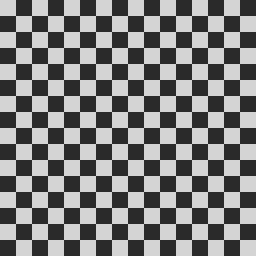
\includegraphics[scale=0.30]{damier.png}}
\subfigure[unidirectional homography $h=h_1 \circ h_2$]{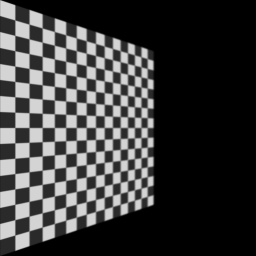
\includegraphics[scale=0.30]{homo_unidirec_f14_2.png}}
\subfigure[transform $h_1$ ]{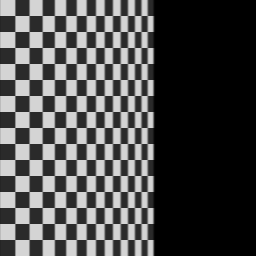
\includegraphics[scale=0.30]{homo_unidirec_part_1_f14_2.png}}
\subfigure[transform $h_2$]{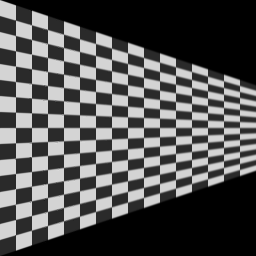
\includegraphics[scale=0.30]{homo_unidirec_part_2_f14_2.png}}
\caption{Separation of a unidirectional homography (scale $0.3$) }
\label{image_separation_f14}
\end{figure}

%\paragraph{Sous-échantillonnage gaussien}
\paragraph{Gaussian downsampling}
\label{zoom_gaussien}
The gaussian zoom is a method of downsampling which uses the convolution $f*G_{d}$, where $G_d$ is a Gaussian kernel of standard deviation $d$. Approximations of the required standard deviation are briefly described in this section, and are based on \emph{is SIFT scale invariant} \cite{morel2011sift}.

%Le zoom gaussien est une méthode de sous-échantillonnage utilisant la convolution $f*G_{d}$ , où $G_d$ est un noyau gaussien d'écart type $d$. Dans nos algorithme on utilisera la méthode développée dans l'article \emph{is SIFT scale invariant} \cite{morel2011sift}.

Let $f$ be an image, assume $f$ is of form $f=G_{c'} * f'$ where $f'$ is an infinite-resolution image. The parameter $c'$ is the Gaussian blur of the image $f$. Experiments show that the ideal blur is $c'=0.8$ \cite{morel2011sift}.\\
Let $z \in [1,+\infty[$, consider $f'_z(x)=f'(zx)$ the downsampled infinite-resolution image.
The Gaussian blur $c$ of the downsampled image $f_z : x \mapsto f(zx)$ has to be $0.8$. To achieve this goal, one may want to convolve $f$ with $G_\sigma$ (with an appropriate standard deviation $\sigma$) before downsample. Since

\begin{equation*}
(f'_z*G_{c})(x)=(f'*G_{cz})(zx)
\end{equation*}
and 
\begin{equation*}
(f*G_\sigma)(zx)=(f'*G_c'*G_\sigma)(zx)=(f'*G_{\sqrt{c'^2 + \sigma^2}})(zx)
\end{equation*}
we conclude
\begin{equation}
\sigma=\sqrt{c^2 z^2 - c'^2}.
\label{formule_zoom_gaussien}
\end{equation}
The parameter $c'$ (the Gaussian blur of the input image) is difficult to compute or to predict. Experiments show that it is between $0.8$ and $0.4$ for reasonably sampled images. A Gaussian blur of $0.7$ in the input image is assumed in our implementation.

%Si $f$ est une image on suppose que $f$ peut s'écrire sous la forme $f=G_{c'} * f'$, où $f'$ est une image de résolution infinie. Le paramètre $c'$ est le facteur de flou gaussien idéal de l'image $f$. L'expérience montre que le facteur de flou gaussien idéal se situe autour de $c=0.8$ \cite{morel2011sift}.\\
%Soit $z\le 1$ posons $f''(x)=f'(zx)$. Si on cherche à échantillonner la fonction  $x\mapsto f(zx)$,  on doit d'abord s'assurer qu'elle possède un facteur de flou gaussien égal à $0.8$. On sait que 

%Grâce à cette relation, on peut en déduire la valeur de $d$ à utiliser, sachant que l'image de départ possède un flou gaussien de $c'$. On obtient

%En identifiant ces deux expressions, on obtient

%Le paramètre $c'$ est difficile à déterminer en pratique. L'expérience montre que pour une image "correctement échantillonnée", le facteur de zoom doit être pris égal à $0.7$. Cependant, pour certaines images provenant de la photographie, on peut prendre $c'=0.5$.

\paragraph{Resampling using integral images}
%\paragraph{Ré-échantillonnage par les images intégrales}
\label{4Integral}

In this paragraph, a method to resample a unidimensional image is presented. This method relies on an approximation of Gaussian blurs using integral images.%(cf. \ref{zoom_gaussien})

%Dans ce paragraphe on présente une méthode permettant de ré-échantillonner une image 1D ; cette méthode s'appuie sur une approximation du zoom gaussien (cf. \ref{zoom_gaussien}) et utilise les images intégrales.

In the following, we denote $\Gcal_n^d$ the kernel defined by
\begin{equation}
\Gcal_1^d(x)=\frac{1}{d}\mathds{1}_{]-\frac{d}{2},\frac{d}{2}[}(x) \text{ and } \Gcal_{n+1}^d= \Gcal_n^d * \Gcal_1^d .
\label{formule_convol_n_int}
\end{equation}

\begin{prop}
The function $x\mapsto \sqrt{n}~\Gcal_n^d(\sqrt{n}~x)$ converges uniformly on $\mathbb{R}$ to a Gaussian function .
\end{prop}

%Soit $\Gcal_n^d$ le noyau définit par 

%Cette suite de fonctions vérifie la propriété suivante
%\begin{prop}
%La fonction $x\mapsto \sqrt{n}~\Gcal_n^d(\sqrt{n}~x)$ converge uniformément sur $\mathbb{R}$ vers une courbe gaussienne 
%\end{prop}
\begin{figure}
\centering
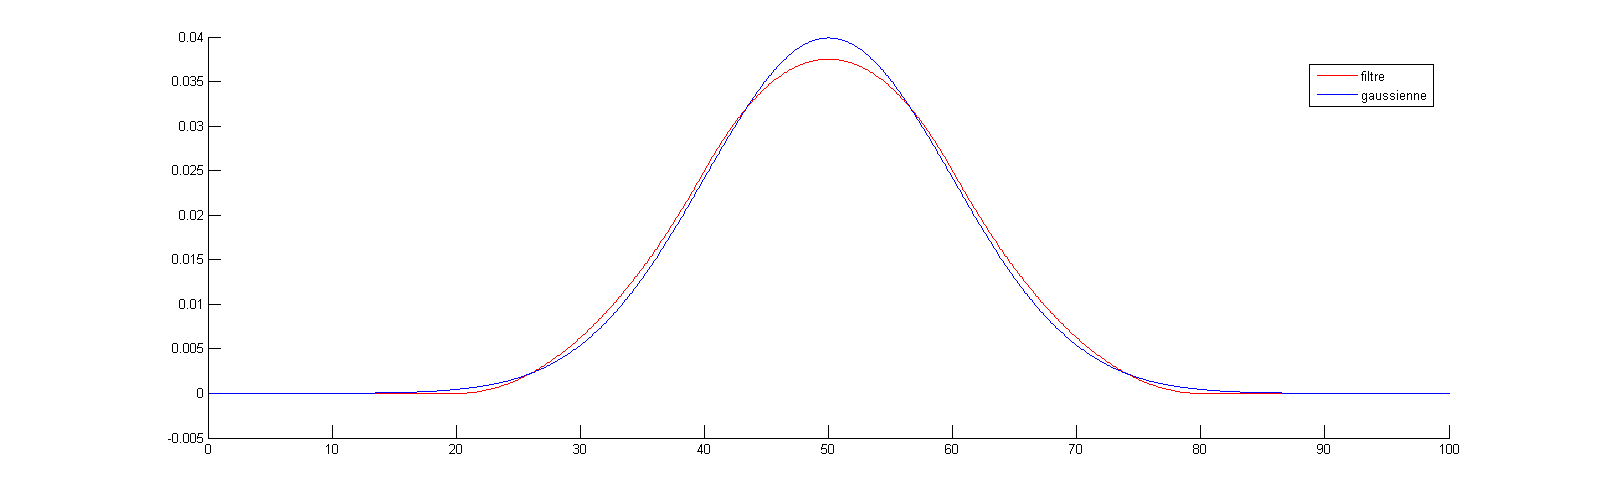
\includegraphics[width=15cm]{filtre_g3.png}
\caption{Comparison between $\Gcal_3^{20}$ and $G_{10}$ (centered on $50$)}
\end{figure}

From now on we denote $D_d$ the ''discret differentiation'' operator defined by $D_d f(x)=\frac{f(x+\frac{d}{2})-f(x-\frac{d}{2})}{d}$ and if $f$ is a compactly supported piecewise continuous function, we denote \begin{equation*}
F_{n+1}(x)= \int_{-\infty}^{x}F_{n}(y)dy~~~ \txt{ and }~~~F_{0}(x)= f(x).
\end{equation*}

Then, we have the following proposition for the continuous case :

\begin{prop} If $f$ is a compactly supported piecewise continuous function then
\begin{equation}
 (f*\Gcal_n^d)(y)=D_d^n F_{n}(y)= \frac{1}{d^n}\underset{0 \le k\le n}{\sum} \binom{n}{k}(-1)^{k} F_{n}(y+\frac{(n-2k)d}{2}).
\end{equation}
\label{continuous_approx}
\end{prop}



%Si $f$ est une fonction continue par morceaux on définit $D_d$ l'opérateur de "dérivation discrète" par $D_d f(x)=\frac{f(x+\frac{d}{2})-f(x-\frac{d}{2})}{d}$  et on pose

%On a alors lemme suivant 

\begin{proof}
Let $f$ be a compactly supported piecewise continuous function, then
\begin{eqnarray*}
(f * \Gcal_1^d )(y)&=&\frac{1}{d} \int_{[y-\frac{d}{2},y+\frac{d}{2}]} f(x) dx\\
               &=&\frac{F_{1}(y+\frac{d}{2})-F_{1}(y-\frac{d}{2})}{d}\\
               &=&D_d F_{1}(y)
\end{eqnarray*}


\noindent Let's prove by induction on $n$ that $ f*\Gcal_n^d=D_d^n F_{n}$.\\
It is true for $n=1$. If it is true for $n$ then
\begin{equation*}
f*\Gcal_{n+1}^{d}=(f * \Gcal_{n}^d) * \Gcal_{1}^{d}= (D_d^n F_{n})*\Gcal_1^d.
\end{equation*}
By linearity of the convolution
\begin{equation*}
(f*\Gcal_{n+1}^{d}) = D_d^n (F_{n}*\Gcal_1^d) = D_d^{n+1} F_{n+1}.
\end{equation*}
$D_d^n$ is the sum of translation operators
\begin{equation*}
f\mapsto f(\cdot+\frac{d}{2})~~~\txt{ and }~~~f\mapsto f(\cdot-\frac{d}{2})?
\end{equation*}
so it can be developed using a binomial formula. Therefore

%On peut développer $D_d^n$ à l'aide du binome de Newton car les deux opérateurs commutent. On obtient donc
\begin{equation*}
(f*\Gcal_n^d)(y) = \frac{1}{d^n}\underset{0 \le k\le n}{\sum} \binom{n}{k}(-1)^{k} F_{n}(y+\frac{(n-2k)d}{2}).
\end{equation*}
\end{proof}


%In the implementation, the computation of $D_d^n$ is done by induction (see algorithm \ref{pseudo_code_convol_4_int}).

An approximation of $F_{k}$ is required in order to adapt proposition \ref{continuous_approx} to a discrete signal and use these formulas.\\
\medbreak
Let $(f_k)_{k=0...m-1}$ be a discrete signal, define $(F_n)$ the piecewise polynomial interpolation of degree $n$ by

\begin{equation}
F_{0} (x) =\underset{0\le k \le m-1}{\sum}f_{k} \mathds{1}_{[k,k+1[}(x) \txt{ and }  F_{n}(x)=\int_{-\infty}^{x}F_{n-1}(y)dx.
\label{defintion_fn}
\end{equation}

\noindent Then $F_{n}$ can be computed for every $n\in\mb{N}$ : for $n=1$,

\begin{equation*}
F_{1}(x)=\underset{k\le \lfloor x\rfloor \wedge m-1}{\sum}f_{k}+ f_{\lfloor x\rfloor}
(x-\lfloor x\rfloor)
\end{equation*}

\noindent This function is a piecewise affine map. It can be shown by induction on $n\geq 1$ that

\begin{eqnarray*}
F_{n}(x)
&=&
F_n(\lfloor x\rfloor) + \displaystyle{\sum_{0 \leq k \leq n-1}}F_{k}(\lfloor x \rfloor) \frac{(x-\lfloor x \rfloor)^{n-k}}{(n-k)!} \text{ if } x<m\\
&=&
F_{n}(m) + \displaystyle{\sum_{1 \leq k \leq n-1}} F_{k}(m) \frac{(x-m)^{n-1-k}}{(n-1-k)!} \text{ if } x \geq m
\end{eqnarray*}

\noindent where values of $F_n(\lfloor x\rfloor)$ can be computed by induction using

\begin{equation*}
\forall k \in \llbracket 0 ; m-1 \rrbracket, F_{n}(k+1)=F_{n}(k)+\underset{0\le l \leq n-1}{\sum} \frac{F_{l}(k)}{(n-l)!}
\end{equation*}

%Dans nos algorithmes, on utilisera généralement cette propriété pour $n=3$ mais on calculera l'opérateur $D_d^n$ en faisant des différences successives (algorithme \ref{pseudo_code_convol_4_int}).

%On doit cependant calculer une valeur approchée des fonctions $F_{k}$  car on ne connait que les échantillons de la fonctions $f$.\\
%Si le signal discret possède $m$ valeurs non nulles $f_k,k=0...m-1$, on peut poser 


%Cette fonction est affine par morceaux. On peut démontrer la formule suivante par récurrence

%Où la valeur de $F_{n}$ se calcule par récurrence :

\noindent So the values on integers and the value of a polynomial of degree $n$ has to be computed to interpolate on non-integers.

\medbreak
With this method the signal $(f_k)$ could be resampled by interpolating it with $F_{0}$ in the first place, and then by convolving with a kernel $\Gcal_n^d$.

\noindent But when this method is used, the image is initially interpolated with a piecewise constant function, and when $d$ is small, resampling using $F_{0}*\Gcal_n^d$ is equivalent to resampling using the value of the closest point. However this problem can be solved by convolving initially with $\Gcal_1^1$, and therefore considering a piecewise affine interpolation $\tilde F = F_0*\Gcal_1^1$ of the samples $(f_k)$.

%Dans cette méthode on ré-échantillonne le signal $(f_k)$ en l'interpolant d'abord par la fonction $F_{0}$, puis on ré-échantillonne en appliquant une convolution avec un noyau $\Gcal_n^d$. On utilise dans nos algorithmes les fonctions $\Gcal_3^d$ car elles se sont de bonnes approximations de courbes gaussiennes.\\ %placer figure 
%Dans cette méthode, l'image est initialement interpolée par une fonction constante par morceaux. Lorsque le paramètre $d$ est choisi très petit, le ré-échantillonnage $F_{0}*\Gcal_3^d$ est équivalent à la méthode du point le plus proche.\\
%On peut cependant corriger ce problème


%JUJUJU

\begin{prop}
Let $(f_k)$ be a discrete signal, $(F_n)$ defined by \eqref{defintion_fn} and $\tilde F$ its piecewise affine interpolation. Then
\begin{equation*}
( \tilde{F} * \Gcal_n^d ) (x) = D_d^{n}D_1 F_{n+1}(x).
\end{equation*}
\end{prop}

\begin{proof}
We have
\begin{equation*}
\tilde{F}(x)=(F_{0} * \Gcal_1^1 )(x),
\end{equation*}
so
\begin{equation*}
\tilde{F}*\Gcal_n^d=F_{0}*\Gcal_1^1*\Gcal_n^d=F_{0}*\Gcal_n^d*\Gcal_1^1=(D_d^n F_{n})*\Gcal_1^1=D_d^n (F_{n}*\Gcal_1^1)= D_d^n (D_1 F_{n+1}).
\end{equation*}
\end{proof}


The additional interpolation can be obtained by evaluating $F_{n+1}$.
It is possible to use this method to have a more regular representation of the input signal, but $F_0 * \Gcal_p^1~$ is not exact on the integers if $2\le p$.\\
In practice the implementation uses $\Gcal_3^d * \Gcal_1^1$, and therefore approximations of $F_n$ for $n=1...4$ are required.



To compute the values of $F_n$ for $n=1...4$, values on integers are precomputed and then polynomials are evaluated.


To precompute the values on integers, the relations
\begin{eqnarray}
F_{1}(k+1)&=&  F_{1}(k)+f_{k}, \label{formula_discret_integral_1}\\
F_{2}(k+1)&=&  F_{2}(k)+F_{1}(k)+\frac{f_{k}}{2}, \label{formula_discret_integral_2}\\
F_{3}(k+1)&=&  F_{3}(k)+F_{2}(k)+\frac{F_{1}(k)}{2}+\frac{f_{k}}{6}, \label{formula_discret_integral_3}\\
F_{4}(k+1)&=&  F_{4}(k)+F_{3}(k)+\frac{F_{2}(k)}{2}+\frac{F_{1}(k)}{6}+\frac{f_{k}}{24}, \label{formula_discret_integral_4}
\end{eqnarray}
are used (see algorithm \ref{pseudo_code_built_4_int}).


%On doit calculer une composante constante par morceaux afin d'avoir la valeur de $F_{n}$ aux entiers ainsi qu'un terme polynomial de degré $n$ pour effectuer l'interpolation sur des valeurs non-entières.

To compute values on non-integers, the following scheme is used :

\begin{itemize}
\item If $x\le 0$ then
\begin{equation}
\label{formula_nonint_integral_case1}
F_{4}(x)=0.
\end{equation}
\item If $x\in ]0 , m[$ then
\begin{equation}
\label{formula_nonint_integral_case2}
F_{4}(x)-F_{4}(\lfloor x \rfloor)=P_{\lfloor x \rfloor}(x-\lfloor x \rfloor)
\end{equation}
where $P_k$ is a polynomial of degree $4$ defined by
\begin{equation*}
P_k (r) =r \left( F_{3}(k) +\frac{r}{2} \left(F_{2}(k)+ \frac{r}{3}\left(F_{1}(k)+\frac{r}{4} f_{k}\right)\right)\right), k=0...m-1.
\end{equation*}
\item If $x\ge m$ then
\begin{equation}
\label{formula_nonint_integral_case3}
F_{4}(x)-F_{4}(m)=Q(x-m)
\end{equation}
where  $Q$ is a polynomial of degree 3 defined by
\begin{equation*}
Q(r)=r \left(F_{3}(m)+\frac{r}{2} \left( F_{2}(m) + \frac{r}{3} F_1 (m)\right)\right).
\end{equation*}\
\end{itemize}

These formulas are used in the algorithm \ref{pseudo_code_eval_4_int}.

%Dans la pratique, on a utilisé cette formule pour $n=4$. Afin d'évaluer $F_4$, on procède de la façon suivante 

%Ces formules sont utilisées dans l'algorithme permettant d'évaluer l'intégrale quatrième de l'image (algorithme \ref{pseudo_code_eval_4_int}).

%Pour calculer la valeur $F_4$ aux entiers, on peut applique la relation de récurrence suivante

%Ces formules sont utilisées dans le pseudo-code (algorithme \ref{pseudo_code_built_4_int}).


\medbreak


To implement this method, the parameter $d$ has to be chosen with respect to the local zoom $z$ in the point considered. The zoom factor $z$ is given by the derivative of the transform.\\
The results from the previous paragraph (cf. \ref{zoom_gaussien}) are used since $\Gcal_3^d$ is a good approximation of a Gaussian function. According to Wells \cite{wells1986efficient}, the parameter $d$ so that $\Gcal_3^d$ approximates $G_\sigma$ should check $\sigma^2 = \frac 1 4 \left((d+1)^2-1\right)$. Thus, for $z \geq 1$, by \eqref{formule_zoom_gaussien}

\begin{equation*}
d=\sqrt{2(c^2 z^2 - c'^2)+1}-1 \text{ with } c=0.8 \text{ and } c'=0.7.
\end{equation*}

The value of $c'$ is fixed to $0.7$ in our implementation, but it could be chosen accordingly to the input image : for sharp image, it has to be around $0.5$ to avoid aliasing. A too small value introduces an excessive blur.

%L'interpolation supplémentaire peut donc être obtenue en évaluant $F_{n+1}$. La méthode de calcul est donc la même que dans le cas précédent, la convolution avec $\Gcal_3^d$ nécessite l'utilisation l'intégrale quatrième de l'image dans la pratique.\\
%Il est possible d'utiliser cette méthode pour obtenir une représentation plus régulière du signal de départ mais la courbe $F_0 * \Gcal_p^1~$ n'est pas interpolante si $2\le p$.\\
%à faire mieux 
%Afin d'implémenter cette méthode, nous devons déterminer la valeur du paramètre $d$ en fonction du facteur de zoom local $z$ que l'on doit effectuer en ce point. $z$ sera choisi égal à la dérivé de la transformation au point où l'on ré-échantillonne.\\ 
%On réutilise les résultats du paragraphe précédent (cf. \ref{zoom_gaussien}), car les  fonctions $\Gcal_3^d$ sont de bonnes approximations de courbes gaussiennes. L'écart type $\sigma$ de $\Gcal_3^d$ est donné par la formule 

%Par la formule du zoom gaussien (formule \ref{formule_zoom_gaussien}), on en déduit que si $z\ge 1$, alors

%La valeur de $c'$ peut être choisie en fonction de l'image d'entrée : pour des images très nettes, si l'on souhaite que le résultat final ne soit pas aliasé, on doit prendre une valeur de $c'$ autour de $0.5$. Pour la majorité des image utilisée lors de nos expériences une valeur de $0.7$ était suffisante. Une valeur trop faible de $c'$ aboutit à un flou excessif.
